% 2015-05-21 - Emerson Ribeiro de Mello - mello@ifsc.edu.br
% \documentclass[handout,xcolor=pdftex,dvipsnames,table]{beamer}
\documentclass{beamer}

\usepackage[utf8]{inputenc}
\usepackage[T1]{fontenc}
\usepackage[english,brazil]{babel}

\usepackage{blindtext}


% usando tema personalizado. 
% arquivo beamerthemeIFSC.sty deve estar no mesmo diretório do .tex
\usepackage{beamerthemeIFSC}


\hypersetup{pdfstartview={Fit},pdftitle={\@title},
 	pdfsubject={Introduction to MATLAB},pdfauthor={\@author}
}



%%%%%%%%%%%%%%%%%%%%%%%%%%%%%%%%%%%%%%%%%%%%


\title{Introduction to MATLAB}
\author{Ahmad Asadi}
\date{Spring 2016}
\institute{Amirkabir University of Technology\\
Department of Computer Engineering and Information Technology\\
\url{ahmad.asadi@aut.ac.ir}
}



%%%%%%%%%%%%%%%%%%%%%%%%%%%%%%%%%%%%%%%%%%%%

\begin{document}

\begin{frame}[t]
	\maketitle
\end{frame}

% Descomente as linhas abaixo se desejar colocar um sumário de todas as seções
\begin{frame}[t]{Outlines}
\tableofcontents
\end{frame}


\def\sectionname{}
\def\insertsectionnumber{}
\def\subsectionname{}
\def\insertsubsectionnumber{}

\AtBeginSection{\frame{\sectionpage}\addtocounter{framenumber}{-1}}


\AtBeginSubsection{\frame{\subsectionpage}\addtocounter{framenumber}{-1} }
\AtBeginSubsubsection{\frame{\subsubsectionpage}\addtocounter{framenumber}{-1} }






%%%%%%%%%%%%%%%%%%%%%%%%%%%%%%%%%%%%%%%%%%%%
% Inicio do documento
%%%%%%%%%%%%%%%%%%%%%%%%%%%%%%%%%%%%%%%%%%%%




\section{Quick Look}


\begin{frame}{\\ What we will see}
	\begin{itemize}
		\item What is MATLAB?
		\item Graphical User Interface of MATLAB
		\item Basic Syntax
	\end{itemize}
\end{frame}

\begin{frame}{\\What is MATLAB?}
	\begin{block}{}
		\begin{itemize}
			\item A high level programming language being used for technical sophisticated computations
			\item Everything is matrix
			\item Stands for: \textit{\textbf{MAT}}rix \textit{\textbf{LAB}}oratory
			\item Can be assumed as a  powerful super calculator 
			\item Matrix based structure $\rightarrow$ awesome to do linear algebra
		\end{itemize}
	\end{block}
	\begin{alertblock}{Note}
		Matlab is extremely broader than what we will cover in this course. We just want to understand its basics.
	\end{alertblock}
\end{frame}


\begin{frame}{Look around MATLAB}
	\begin{block}{Pros}
		\begin{itemize}
			\item Fast and easy prototyping
			\item A wide variety of provided libraries including wide diversity of applications
			\item Great easy graphical display facilities
			\item Providing facilities to quickly make a little tiny application
			\item Quick to learn \& efficient to use
		\end{itemize}
	\end{block}
	\begin{alertblock}{Cons}
		\begin{itemize}
			\item It seems slow for some sort of programs (we will see them later)
			\item A program that is just for personal usages (not available on web, not designed for large scale applications, not designed in a multi-user fashion, etc.)

		\end{itemize}
	\end{alertblock}
\end{frame}


\begin{frame}{\\Applications}
	\begin{block}{}
		\begin{itemize}
			\item Math and Computations
			\item Algorithm Development
			\item Modeling, Simulation and Prototyping
			\item Data Analysis, Exploration and Visualization
			\item Scientific and Engineering Graphics
			\item Optimized mining operations through modeling and simulation
			\item Automated data analysis, processing and reporting
			\item Forecast economical risk and profitability using financial predictive modeling
			\item Almost, one of the most useful handy applications for engineers and also scientists
		\end{itemize}
	\end{block}
\end{frame}


\begin{frame}{\\How to work with MATLAB?}
	\begin{block}{Big Picture}
		\begin{itemize}
			\item Learn Rules (Syntax)
			\item Decompose interesting problem into simple steps
			\item Express each step according to MATLAB syntax
			\item Let MATLAB To do it!
		\end{itemize}
	\end{block}
\end{frame}


\begin{frame}{Graphical User Interface (GUI)}
	\begin{figure}
		\center
		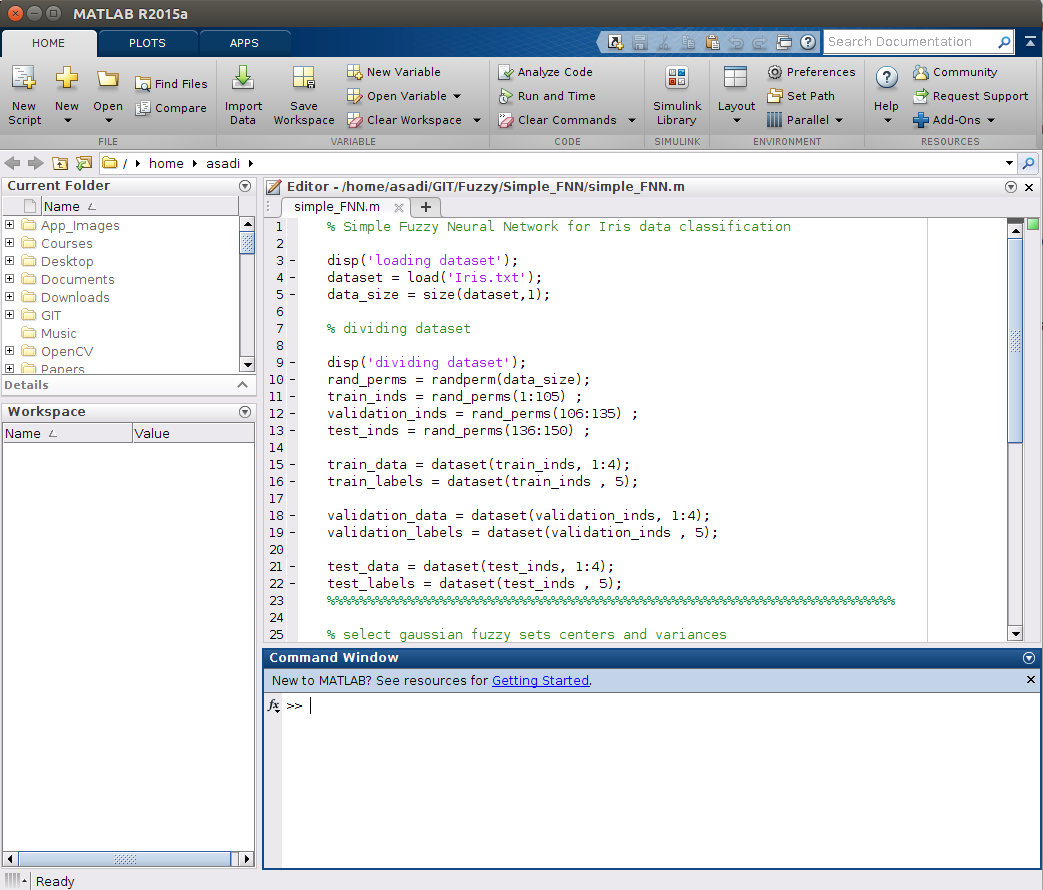
\includegraphics[scale=0.25]{./Imgs/GUI.png}
	\end{figure}
\end{frame}




\subsection{Blocos}


\begin{frame}{Blocos}
	\begin{block}{Esse e um bloco}
		Isso e um teste
	\end{block}
	\begin{block}{}
	Bloco sem titulo	
	\end{block}
	\begin{alertblock}{Alerta}
		Esse e um alerta
	\end{alertblock}
\end{frame}

%parâmetros: linguagem (shell, java, matlab, python, c, php) e arquivo

%\includecode[shell]{codigos/ola.sh}
%
%\includecode[matlab]{codigos/matlab.m}

%ou
% invocar os comandos \ansic, \java, \shell e colocar o código no próprio slide


\begin{frame}[fragile]{Codigo em C e Java}

\includecode[ansic]{codigos/ola.c}	

\ansic
	\begin{lstlisting}
	 int main(void){
	    printf("Ola mundo\n");
	    return 0;
	 }
	\end{lstlisting}
\java
	\begin{lstlisting}
	 public static voi main(String args[]){
	    System.out.println("Ola mundo");
	 }
	\end{lstlisting}	
	
\end{frame}






\end{document}